\documentclass[1p]{elsarticle_modified}
%\bibliographystyle{elsarticle-num}

%\usepackage[colorlinks]{hyperref}
%\usepackage{abbrmath_seonhwa} %\Abb, \Ascr, \Acal ,\Abf, \Afrak
\usepackage{amsfonts}
\usepackage{amssymb}
\usepackage{amsmath}
\usepackage{amsthm}
\usepackage{scalefnt}
\usepackage{amsbsy}
\usepackage{kotex}
\usepackage{caption}
\usepackage{subfig}
\usepackage{color}
\usepackage{graphicx}
\usepackage{xcolor} %% white, black, red, green, blue, cyan, magenta, yellow
\usepackage{float}
\usepackage{setspace}
\usepackage{hyperref}

\usepackage{tikz}
\usetikzlibrary{arrows}

\usepackage{multirow}
\usepackage{array} % fixed length table
\usepackage{hhline}

%%%%%%%%%%%%%%%%%%%%%
\makeatletter
\renewcommand*\env@matrix[1][\arraystretch]{%
	\edef\arraystretch{#1}%
	\hskip -\arraycolsep
	\let\@ifnextchar\new@ifnextchar
	\array{*\c@MaxMatrixCols c}}
\makeatother %https://tex.stackexchange.com/questions/14071/how-can-i-increase-the-line-spacing-in-a-matrix
%%%%%%%%%%%%%%%

\usepackage[normalem]{ulem}

\newcommand{\msout}[1]{\ifmmode\text{\sout{\ensuremath{#1}}}\else\sout{#1}\fi}
%SOURCE: \msout is \stkout macro in https://tex.stackexchange.com/questions/20609/strikeout-in-math-mode

\newcommand{\cancel}[1]{
	\ifmmode
	{\color{red}\msout{#1}}
	\else
	{\color{red}\sout{#1}}
	\fi
}

\newcommand{\add}[1]{
	{\color{blue}\uwave{#1}}
}

\newcommand{\replace}[2]{
	\ifmmode
	{\color{red}\msout{#1}}{\color{blue}\uwave{#2}}
	\else
	{\color{red}\sout{#1}}{\color{blue}\uwave{#2}}
	\fi
}

\newcommand{\Sol}{\mathcal{S}} %segment
\newcommand{\D}{D} %diagram
\newcommand{\A}{\mathcal{A}} %arc


%%%%%%%%%%%%%%%%%%%%%%%%%%%%%5 test

\def\sl{\operatorname{\textup{SL}}(2,\Cbb)}
\def\psl{\operatorname{\textup{PSL}}(2,\Cbb)}
\def\quan{\mkern 1mu \triangleright \mkern 1mu}

\theoremstyle{definition}
\newtheorem{thm}{Theorem}[section]
\newtheorem{prop}[thm]{Proposition}
\newtheorem{lem}[thm]{Lemma}
\newtheorem{ques}[thm]{Question}
\newtheorem{cor}[thm]{Corollary}
\newtheorem{defn}[thm]{Definition}
\newtheorem{exam}[thm]{Example}
\newtheorem{rmk}[thm]{Remark}
\newtheorem{alg}[thm]{Algorithm}

\newcommand{\I}{\sqrt{-1}}
\begin{document}

%\begin{frontmatter}
%
%\title{Boundary parabolic representations of knots up to 8 crossings}
%
%%% Group authors per affiliation:
%\author{Yunhi Cho} 
%\address{Department of Mathematics, University of Seoul, Seoul, Korea}
%\ead{yhcho@uos.ac.kr}
%
%
%\author{Seonhwa Kim} %\fnref{s_kim}}
%\address{Center for Geometry and Physics, Institute for Basic Science, Pohang, 37673, Korea}
%\ead{ryeona17@ibs.re.kr}
%
%\author{Hyuk Kim}
%\address{Department of Mathematical Sciences, Seoul National University, Seoul 08826, Korea}
%\ead{hyukkim@snu.ac.kr}
%
%\author{Seokbeom Yoon}
%\address{Department of Mathematical Sciences, Seoul National University, Seoul, 08826,  Korea}
%\ead{sbyoon15@snu.ac.kr}
%
%\begin{abstract}
%We find all boundary parabolic representation of knots up to 8 crossings.
%
%\end{abstract}
%\begin{keyword}
%    \MSC[2010] 57M25 
%\end{keyword}
%
%\end{frontmatter}

%\linenumbers
%\tableofcontents
%
\newcommand\colored[1]{\textcolor{white}{\rule[-0.35ex]{0.8em}{1.4ex}}\kern-0.8em\color{red} #1}%
%\newcommand\colored[1]{\textcolor{white}{ #1}\kern-2.17ex	\textcolor{white}{ #1}\kern-1.81ex	\textcolor{white}{ #1}\kern-2.15ex\color{red}#1	}

{\Large $\underline{12a_{0502}~(K12a_{0502})}$}

\setlength{\tabcolsep}{10pt}
\renewcommand{\arraystretch}{1.6}
\vspace{1cm}\begin{tabular}{m{100pt}>{\centering\arraybackslash}m{274pt}}
\multirow{5}{120pt}{
	\centering
	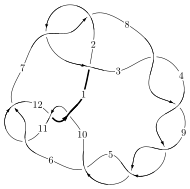
\includegraphics[width=112pt]{../../../GIT/diagram.site/Diagrams/png/1303_12a_0502.png}\\
\ \ \ A knot diagram\footnotemark}&
\allowdisplaybreaks
\textbf{Linearized knot diagam} \\
\cline{2-2}
 &
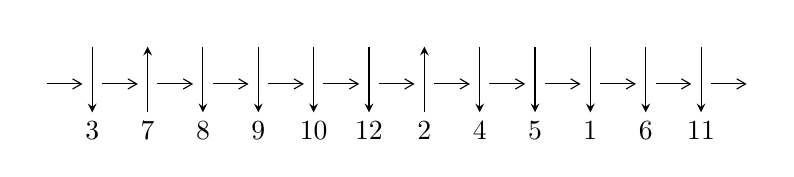
\begin{tikzpicture}[x=20pt, y=17pt]
	% nodes
	\node (C0) at (0, 0) {};
	\node (C1) at (1, 0) {};
	\node (C1U) at (1, +1) {};
	\node (C1D) at (1, -1) {3};

	\node (C2) at (2, 0) {};
	\node (C2U) at (2, +1) {};
	\node (C2D) at (2, -1) {7};

	\node (C3) at (3, 0) {};
	\node (C3U) at (3, +1) {};
	\node (C3D) at (3, -1) {8};

	\node (C4) at (4, 0) {};
	\node (C4U) at (4, +1) {};
	\node (C4D) at (4, -1) {9};

	\node (C5) at (5, 0) {};
	\node (C5U) at (5, +1) {};
	\node (C5D) at (5, -1) {10};

	\node (C6) at (6, 0) {};
	\node (C6U) at (6, +1) {};
	\node (C6D) at (6, -1) {12};

	\node (C7) at (7, 0) {};
	\node (C7U) at (7, +1) {};
	\node (C7D) at (7, -1) {2};

	\node (C8) at (8, 0) {};
	\node (C8U) at (8, +1) {};
	\node (C8D) at (8, -1) {4};

	\node (C9) at (9, 0) {};
	\node (C9U) at (9, +1) {};
	\node (C9D) at (9, -1) {5};

	\node (C10) at (10, 0) {};
	\node (C10U) at (10, +1) {};
	\node (C10D) at (10, -1) {1};

	\node (C11) at (11, 0) {};
	\node (C11U) at (11, +1) {};
	\node (C11D) at (11, -1) {6};

	\node (C12) at (12, 0) {};
	\node (C12U) at (12, +1) {};
	\node (C12D) at (12, -1) {11};
	\node (C13) at (13, 0) {};

	% arrows
	\draw[->,>={angle 60}]
	(C0) edge (C1) (C1) edge (C2) (C2) edge (C3) (C3) edge (C4) (C4) edge (C5) (C5) edge (C6) (C6) edge (C7) (C7) edge (C8) (C8) edge (C9) (C9) edge (C10) (C10) edge (C11) (C11) edge (C12) (C12) edge (C13) ;	\draw[->,>=stealth]
	(C1U) edge (C1D) (C2D) edge (C2U) (C3U) edge (C3D) (C4U) edge (C4D) (C5U) edge (C5D) (C6U) edge (C6D) (C7D) edge (C7U) (C8U) edge (C8D) (C9U) edge (C9D) (C10U) edge (C10D) (C11U) edge (C11D) (C12U) edge (C12D) ;
	\end{tikzpicture} \\
\hhline{~~} \\& 
\textbf{Solving Sequence} \\ \cline{2-2} 
 &
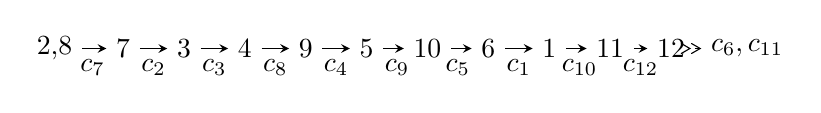
\begin{tikzpicture}[x=22pt, y=7pt]
	% node
	\node (A0) at (-1/8, 0) {2,8};
	\node (A1) at (1, 0) {7};
	\node (A2) at (2, 0) {3};
	\node (A3) at (3, 0) {4};
	\node (A4) at (4, 0) {9};
	\node (A5) at (5, 0) {5};
	\node (A6) at (6, 0) {10};
	\node (A7) at (7, 0) {6};
	\node (A8) at (8, 0) {1};
	\node (A9) at (9, 0) {11};
	\node (A10) at (10, 0) {12};
	\node (C1) at (1/2, -1) {$c_{7}$};
	\node (C2) at (3/2, -1) {$c_{2}$};
	\node (C3) at (5/2, -1) {$c_{3}$};
	\node (C4) at (7/2, -1) {$c_{8}$};
	\node (C5) at (9/2, -1) {$c_{4}$};
	\node (C6) at (11/2, -1) {$c_{9}$};
	\node (C7) at (13/2, -1) {$c_{5}$};
	\node (C8) at (15/2, -1) {$c_{1}$};
	\node (C9) at (17/2, -1) {$c_{10}$};
	\node (C10) at (19/2, -1) {$c_{12}$};
	\node (A11) at (45/4, 0) {$c_{6},c_{11}$};

	% edge
	\draw[->,>=stealth]	
	(A0) edge (A1) (A1) edge (A2) (A2) edge (A3) (A3) edge (A4) (A4) edge (A5) (A5) edge (A6) (A6) edge (A7) (A7) edge (A8) (A8) edge (A9) (A9) edge (A10) ;
	\draw[->>,>={angle 60}]	
	(A10) edge (A11);
\end{tikzpicture} \\ 

\end{tabular} \\

\footnotetext{
The image of knot diagram is generated by the software ``\textbf{Draw programme}" developed by Andrew Bartholomew(\url{http://www.layer8.co.uk/maths/draw/index.htm\#Running-draw}), where we modified some parts for our purpose(\url{https://github.com/CATsTAILs/LinksPainter}).
}\phantom \\ \newline 
\centering \textbf{Ideals for irreducible components\footnotemark of $X_{\text{par}}$} 
 
\begin{align*}
I^u_{1}&=\langle 
u^{45}- u^{44}+\cdots-3 u+1\rangle \\
\\
\end{align*}
\raggedright * 1 irreducible components of $\dim_{\mathbb{C}}=0$, with total 45 representations.\\
\footnotetext{All coefficients of polynomials are rational numbers. But the coefficients are sometimes approximated in decimal forms when there is not enough margin.}
\newpage
\renewcommand{\arraystretch}{1}
\centering \section*{I. $I^u_{1}= \langle u^{45}- u^{44}+\cdots-3 u+1 \rangle$}
\flushleft \textbf{(i) Arc colorings}\\
\begin{tabular}{m{7pt} m{180pt} m{7pt} m{180pt} }
\flushright $a_{2}=$&$\begin{pmatrix}0\\u\end{pmatrix}$ \\
\flushright $a_{8}=$&$\begin{pmatrix}1\\0\end{pmatrix}$ \\
\flushright $a_{7}=$&$\begin{pmatrix}1\\u^2\end{pmatrix}$ \\
\flushright $a_{3}=$&$\begin{pmatrix}u\\u^3+u\end{pmatrix}$ \\
\flushright $a_{4}=$&$\begin{pmatrix}- u^3\\u^3+u\end{pmatrix}$ \\
\flushright $a_{9}=$&$\begin{pmatrix}- u^6- u^4+1\\u^6+2 u^4+u^2\end{pmatrix}$ \\
\flushright $a_{5}=$&$\begin{pmatrix}u^9+2 u^7+u^5-2 u^3- u\\- u^9-3 u^7-3 u^5+u\end{pmatrix}$ \\
\flushright $a_{10}=$&$\begin{pmatrix}u^{12}+3 u^{10}+3 u^8-2 u^6-4 u^4- u^2+1\\- u^{12}-4 u^{10}-6 u^8-2 u^6+3 u^4+2 u^2\end{pmatrix}$ \\
\flushright $a_{6}=$&$\begin{pmatrix}- u^{15}-4 u^{13}-6 u^{11}+8 u^7+6 u^5-2 u^3-2 u\\u^{15}+5 u^{13}+10 u^{11}+7 u^9-4 u^7-8 u^5-2 u^3+u\end{pmatrix}$ \\
\flushright $a_{1}=$&$\begin{pmatrix}u^3\\u^5+u^3+u\end{pmatrix}$ \\
\flushright $a_{11}=$&$\begin{pmatrix}u^{20}+5 u^{18}+11 u^{16}+10 u^{14}-7 u^{10}-3 u^8-2 u^6-3 u^4- u^2+1\\u^{22}+6 u^{20}+\cdots+4 u^4+3 u^2\end{pmatrix}$ \\
\flushright $a_{12}=$&$\begin{pmatrix}u^{37}+10 u^{35}+\cdots-9 u^5+u\\u^{39}+11 u^{37}+\cdots+4 u^3+u\end{pmatrix}$\\&\end{tabular}
\flushleft \textbf{(ii) Obstruction class $= -1$}\\~\\
\flushleft \textbf{(iii) Cusp Shapes $= -4 u^{43}+4 u^{42}+\cdots+20 u-18$}\\~\\
\newpage\renewcommand{\arraystretch}{1}
\flushleft \textbf{(iv) u-Polynomials at the component}\newline \\
\begin{tabular}{m{50pt}|m{274pt}}
Crossings & \hspace{64pt}u-Polynomials at each crossing \\
\hline $$\begin{aligned}c_{1}\end{aligned}$$&$\begin{aligned}
&u^{45}+27 u^{44}+\cdots+3 u-1
\end{aligned}$\\
\hline $$\begin{aligned}c_{2},c_{7}\end{aligned}$$&$\begin{aligned}
&u^{45}+u^{44}+\cdots-3 u-1
\end{aligned}$\\
\hline $$\begin{aligned}c_{3},c_{4},c_{5}\\c_{8},c_{9}\end{aligned}$$&$\begin{aligned}
&u^{45}- u^{44}+\cdots+11 u-1
\end{aligned}$\\
\hline $$\begin{aligned}c_{6},c_{11}\end{aligned}$$&$\begin{aligned}
&u^{45}+u^{44}+\cdots-3 u-1
\end{aligned}$\\
\hline $$\begin{aligned}c_{10},c_{12}\end{aligned}$$&$\begin{aligned}
&u^{45}+17 u^{44}+\cdots+3 u+1
\end{aligned}$\\
\hline
\end{tabular}\\~\\
\newpage\renewcommand{\arraystretch}{1}
\flushleft \textbf{(v) Riley Polynomials at the component}\newline \\
\begin{tabular}{m{50pt}|m{274pt}}
Crossings & \hspace{64pt}Riley Polynomials at each crossing \\
\hline $$\begin{aligned}c_{1}\end{aligned}$$&$\begin{aligned}
&y^{45}-17 y^{44}+\cdots+55 y-1
\end{aligned}$\\
\hline $$\begin{aligned}c_{2},c_{7}\end{aligned}$$&$\begin{aligned}
&y^{45}+27 y^{44}+\cdots+3 y-1
\end{aligned}$\\
\hline $$\begin{aligned}c_{3},c_{4},c_{5}\\c_{8},c_{9}\end{aligned}$$&$\begin{aligned}
&y^{45}-61 y^{44}+\cdots+99 y-1
\end{aligned}$\\
\hline $$\begin{aligned}c_{6},c_{11}\end{aligned}$$&$\begin{aligned}
&y^{45}-17 y^{44}+\cdots+3 y-1
\end{aligned}$\\
\hline $$\begin{aligned}c_{10},c_{12}\end{aligned}$$&$\begin{aligned}
&y^{45}+23 y^{44}+\cdots-17 y-1
\end{aligned}$\\
\hline
\end{tabular}\\~\\
\newpage\flushleft \textbf{(vi) Complex Volumes and Cusp Shapes}
$$\begin{array}{c|c|c}  
\text{Solutions to }I^u_{1}& \I (\text{vol} + \sqrt{-1}CS) & \text{Cusp shape}\\
 \hline 
\begin{aligned}
u &= \phantom{-}0.427459 + 0.911225 I\end{aligned}
 & \phantom{-}0.85804 + 6.50089 I & -8.32802 - 9.97393 I \\ \hline\begin{aligned}
u &= \phantom{-}0.427459 - 0.911225 I\end{aligned}
 & \phantom{-}0.85804 - 6.50089 I & -8.32802 + 9.97393 I \\ \hline\begin{aligned}
u &= \phantom{-}0.070383 + 1.016090 I\end{aligned}
 & -1.72179 - 2.04025 I & -15.9831 + 3.0595 I \\ \hline\begin{aligned}
u &= \phantom{-}0.070383 - 1.016090 I\end{aligned}
 & -1.72179 + 2.04025 I & -15.9831 - 3.0595 I \\ \hline\begin{aligned}
u &= -0.408478 + 0.865533 I\end{aligned}
 & \phantom{-}1.39393 - 1.34908 I & -6.37203 + 4.08552 I \\ \hline\begin{aligned}
u &= -0.408478 - 0.865533 I\end{aligned}
 & \phantom{-}1.39393 + 1.34908 I & -6.37203 - 4.08552 I \\ \hline\begin{aligned}
u &= \phantom{-}0.283223 + 1.012980 I\end{aligned}
 & -3.30573 + 2.64852 I & -17.4700 - 5.8251 I \\ \hline\begin{aligned}
u &= \phantom{-}0.283223 - 1.012980 I\end{aligned}
 & -3.30573 - 2.64852 I & -17.4700 + 5.8251 I \\ \hline\begin{aligned}
u &= \phantom{-}0.935027\phantom{ +0.000000I}\end{aligned}
 & -15.9659\phantom{ +0.000000I} & -15.5090\phantom{ +0.000000I} \\ \hline\begin{aligned}
u &= \phantom{-}0.930328 + 0.019398 I\end{aligned}
 & -11.70540 - 7.28312 I & -11.98320 + 4.60308 I \\ \hline\begin{aligned}
u &= \phantom{-}0.930328 - 0.019398 I\end{aligned}
 & -11.70540 + 7.28312 I & -11.98320 - 4.60308 I \\ \hline\begin{aligned}
u &= -0.923476 + 0.012954 I\end{aligned}
 & -10.00250 + 1.76256 I & -9.73819 - 0.10950 I \\ \hline\begin{aligned}
u &= -0.923476 - 0.012954 I\end{aligned}
 & -10.00250 - 1.76256 I & -9.73819 + 0.10950 I \\ \hline\begin{aligned}
u &= -0.208200 + 0.833837 I\end{aligned}
 & -0.603828 - 1.131350 I & -7.84077 + 5.39431 I \\ \hline\begin{aligned}
u &= -0.208200 - 0.833837 I\end{aligned}
 & -0.603828 + 1.131350 I & -7.84077 - 5.39431 I \\ \hline\begin{aligned}
u &= \phantom{-}0.358679 + 1.138370 I\end{aligned}
 & -4.13553 + 2.70881 I & -12.96314 - 3.74313 I \\ \hline\begin{aligned}
u &= \phantom{-}0.358679 - 1.138370 I\end{aligned}
 & -4.13553 - 2.70881 I & -12.96314 + 3.74313 I \\ \hline\begin{aligned}
u &= \phantom{-}0.440538 + 1.122380 I\end{aligned}
 & -3.51671 + 4.84200 I & -11.51709 - 4.49120 I \\ \hline\begin{aligned}
u &= \phantom{-}0.440538 - 1.122380 I\end{aligned}
 & -3.51671 - 4.84200 I & -11.51709 + 4.49120 I \\ \hline\begin{aligned}
u &= -0.347703 + 1.175290 I\end{aligned}
 & -5.60707 + 2.21593 I & -15.5378 - 1.9663 I \\ \hline\begin{aligned}
u &= -0.347703 - 1.175290 I\end{aligned}
 & -5.60707 - 2.21593 I & -15.5378 + 1.9663 I \\ \hline\begin{aligned}
u &= -0.458823 + 1.138270 I\end{aligned}
 & -4.76002 - 10.14720 I & -13.4545 + 9.2635 I \\ \hline\begin{aligned}
u &= -0.458823 - 1.138270 I\end{aligned}
 & -4.76002 + 10.14720 I & -13.4545 - 9.2635 I \\ \hline\begin{aligned}
u &= -0.411367 + 1.171030 I\end{aligned}
 & -9.02942 - 4.07847 I & -18.7916 + 4.0511 I \\ \hline\begin{aligned}
u &= -0.411367 - 1.171030 I\end{aligned}
 & -9.02942 + 4.07847 I & -18.7916 - 4.0511 I \\ \hline\begin{aligned}
u &= -0.723185\phantom{ +0.000000I}\end{aligned}
 & -5.63052\phantom{ +0.000000I} & -15.3580\phantom{ +0.000000I} \\ \hline\begin{aligned}
u &= -0.705456 + 0.119537 I\end{aligned}
 & -1.83649 + 5.83150 I & -10.37227 - 5.87935 I \\ \hline\begin{aligned}
u &= -0.705456 - 0.119537 I\end{aligned}
 & -1.83649 - 5.83150 I & -10.37227 + 5.87935 I \\ \hline\begin{aligned}
u &= -0.399313 + 0.551155 I\end{aligned}
 & \phantom{-}2.22533 - 2.24395 I & -3.65717 + 3.92179 I \\ \hline\begin{aligned}
u &= -0.399313 - 0.551155 I\end{aligned}
 & \phantom{-}2.22533 + 2.24395 I & -3.65717 - 3.92179 I\\
 \hline 
 \end{array}$$\newpage$$\begin{array}{c|c|c}  
\text{Solutions to }I^u_{1}& \I (\text{vol} + \sqrt{-1}CS) & \text{Cusp shape}\\
 \hline 
\begin{aligned}
u &= \phantom{-}0.644426 + 0.110335 I\end{aligned}
 & -0.671592 - 0.750914 I & -8.28728 + 0.79803 I \\ \hline\begin{aligned}
u &= \phantom{-}0.644426 - 0.110335 I\end{aligned}
 & -0.671592 + 0.750914 I & -8.28728 - 0.79803 I \\ \hline\begin{aligned}
u &= -0.482704 + 1.275130 I\end{aligned}
 & -13.8679 - 6.7706 I & \phantom{-0.000000 } 0 \\ \hline\begin{aligned}
u &= -0.482704 - 1.275130 I\end{aligned}
 & -13.8679 + 6.7706 I & \phantom{-0.000000 } 0 \\ \hline\begin{aligned}
u &= -0.467992 + 1.280780 I\end{aligned}
 & -13.9791 - 3.1742 I & \phantom{-0.000000 } 0 \\ \hline\begin{aligned}
u &= -0.467992 - 1.280780 I\end{aligned}
 & -13.9791 + 3.1742 I & \phantom{-0.000000 } 0 \\ \hline\begin{aligned}
u &= \phantom{-}0.487764 + 1.277220 I\end{aligned}
 & -15.5609 + 12.3367 I & \phantom{-0.000000 } 0 \\ \hline\begin{aligned}
u &= \phantom{-}0.487764 - 1.277220 I\end{aligned}
 & -15.5609 - 12.3367 I & \phantom{-0.000000 } 0 \\ \hline\begin{aligned}
u &= \phantom{-}0.465467 + 1.286340 I\end{aligned}
 & -15.7305 - 2.3351 I & \phantom{-0.000000 } 0 \\ \hline\begin{aligned}
u &= \phantom{-}0.465467 - 1.286340 I\end{aligned}
 & -15.7305 + 2.3351 I & \phantom{-0.000000 } 0 \\ \hline\begin{aligned}
u &= \phantom{-}0.428207 + 0.461832 I\end{aligned}
 & \phantom{-}2.03862 - 2.79869 I & -4.43613 + 3.54362 I \\ \hline\begin{aligned}
u &= \phantom{-}0.428207 - 0.461832 I\end{aligned}
 & \phantom{-}2.03862 + 2.79869 I & -4.43613 - 3.54362 I \\ \hline\begin{aligned}
u &= \phantom{-}0.478105 + 1.284620 I\end{aligned}
 & \phantom{-}19.5602 + 5.0232 I & \phantom{-0.000000 } 0 \\ \hline\begin{aligned}
u &= \phantom{-}0.478105 - 1.284620 I\end{aligned}
 & \phantom{-}19.5602 - 5.0232 I & \phantom{-0.000000 } 0 \\ \hline\begin{aligned}
u &= \phantom{-}0.386025\phantom{ +0.000000I}\end{aligned}
 & -0.813684\phantom{ +0.000000I} & -12.1660\phantom{ +0.000000I}\\
 \hline 
 \end{array}$$\newpage
\newpage\renewcommand{\arraystretch}{1}
\centering \section*{ II. u-Polynomials}
\begin{tabular}{m{50pt}|m{274pt}}
Crossings & \hspace{64pt}u-Polynomials at each crossing \\
\hline $$\begin{aligned}c_{1}\end{aligned}$$&$\begin{aligned}
&u^{45}+27 u^{44}+\cdots+3 u-1
\end{aligned}$\\
\hline $$\begin{aligned}c_{2},c_{7}\end{aligned}$$&$\begin{aligned}
&u^{45}+u^{44}+\cdots-3 u-1
\end{aligned}$\\
\hline $$\begin{aligned}c_{3},c_{4},c_{5}\\c_{8},c_{9}\end{aligned}$$&$\begin{aligned}
&u^{45}- u^{44}+\cdots+11 u-1
\end{aligned}$\\
\hline $$\begin{aligned}c_{6},c_{11}\end{aligned}$$&$\begin{aligned}
&u^{45}+u^{44}+\cdots-3 u-1
\end{aligned}$\\
\hline $$\begin{aligned}c_{10},c_{12}\end{aligned}$$&$\begin{aligned}
&u^{45}+17 u^{44}+\cdots+3 u+1
\end{aligned}$\\
\hline
\end{tabular}\newpage\renewcommand{\arraystretch}{1}
\centering \section*{ III. Riley Polynomials}
\begin{tabular}{m{50pt}|m{274pt}}
Crossings & \hspace{64pt}Riley Polynomials at each crossing \\
\hline $$\begin{aligned}c_{1}\end{aligned}$$&$\begin{aligned}
&y^{45}-17 y^{44}+\cdots+55 y-1
\end{aligned}$\\
\hline $$\begin{aligned}c_{2},c_{7}\end{aligned}$$&$\begin{aligned}
&y^{45}+27 y^{44}+\cdots+3 y-1
\end{aligned}$\\
\hline $$\begin{aligned}c_{3},c_{4},c_{5}\\c_{8},c_{9}\end{aligned}$$&$\begin{aligned}
&y^{45}-61 y^{44}+\cdots+99 y-1
\end{aligned}$\\
\hline $$\begin{aligned}c_{6},c_{11}\end{aligned}$$&$\begin{aligned}
&y^{45}-17 y^{44}+\cdots+3 y-1
\end{aligned}$\\
\hline $$\begin{aligned}c_{10},c_{12}\end{aligned}$$&$\begin{aligned}
&y^{45}+23 y^{44}+\cdots-17 y-1
\end{aligned}$\\
\hline
\end{tabular}
\vskip 2pc
\end{document}